%%\subsection{} \label{subsec:revisão}
%
%
%Esta revisão sistemática da literatura aborda o tema das séries temporais, que é de grande relevância em diversas áreas. A seleção dos artigos foi baseada em critérios específicos, levando em consideração a relevância dos autores, os anos de atividade, os países com maior número de publicações e as palavras-chave mais frequentes.
%
%
%
%Embora nem todos os artigos revisados tenham uma forte relação com aprendizado de máquina, eles contribuem cientificamente para este trabalho e podem servir como base para outros pesquisadores.
%
%\begin{figure}[H]
%	\centering
%	\caption{Fluxograma do problema de pesquisa}
%	\label{fig:serie-temporal}
%	\includegraphics[width=1\linewidth]{Revisao/Figuras/"Série temporal"}
%	
%	\fonte{Elaboração própria} 
%\end{figure}
%
%
%A Figura \ref{fig:serie-temporal} apresenta um mapa conceitual das publicações, destacando a importância dos autores como base para esta revisão. Os modelos propostos por esses autores são fundamentais para abordar o problema em questão, uma vez que a previsão em séries temporais é um desafio de grande significado por si só.
%
%
%As questões de pesquisa definidas para esta revisão sistemática da literatura são as seguintes:
%
%\begin{enumerate}[start=1, label = {\textbf{Q} \arabic*} ]
%	\item \label{questão:rev1} Quais são os autores que mais publicam sobre o assunto de séries temporais?
%	\item \label{questão:rev2} Quais são os países que mais publicam sobre o assunto? 
%	\item \label{questão:rev3} Quais são as áreas que mais publicam sobre o tema?
%	\item \label{questão:rev4} Quais são as obras mais influentes na análise de séries temporais?
%\end{enumerate}
%
%
%
%
%
%
%
%
%A Figura \ref{fig:rsl} apresenta uma adaptação da metodologia proposta por \citeonline{MARTINS201671} para a realização desta revisão sistemática. Inicialmente, foram realizadas buscas nos bancos de dados Scopus e Web of Science, selecionando algumas bases relevantes para o tema da pesquisa.
%
%\begin{figure}[H]
%	\centering
%	\caption{Etapas da Revisão}
%	\label{fig:rsl}
%	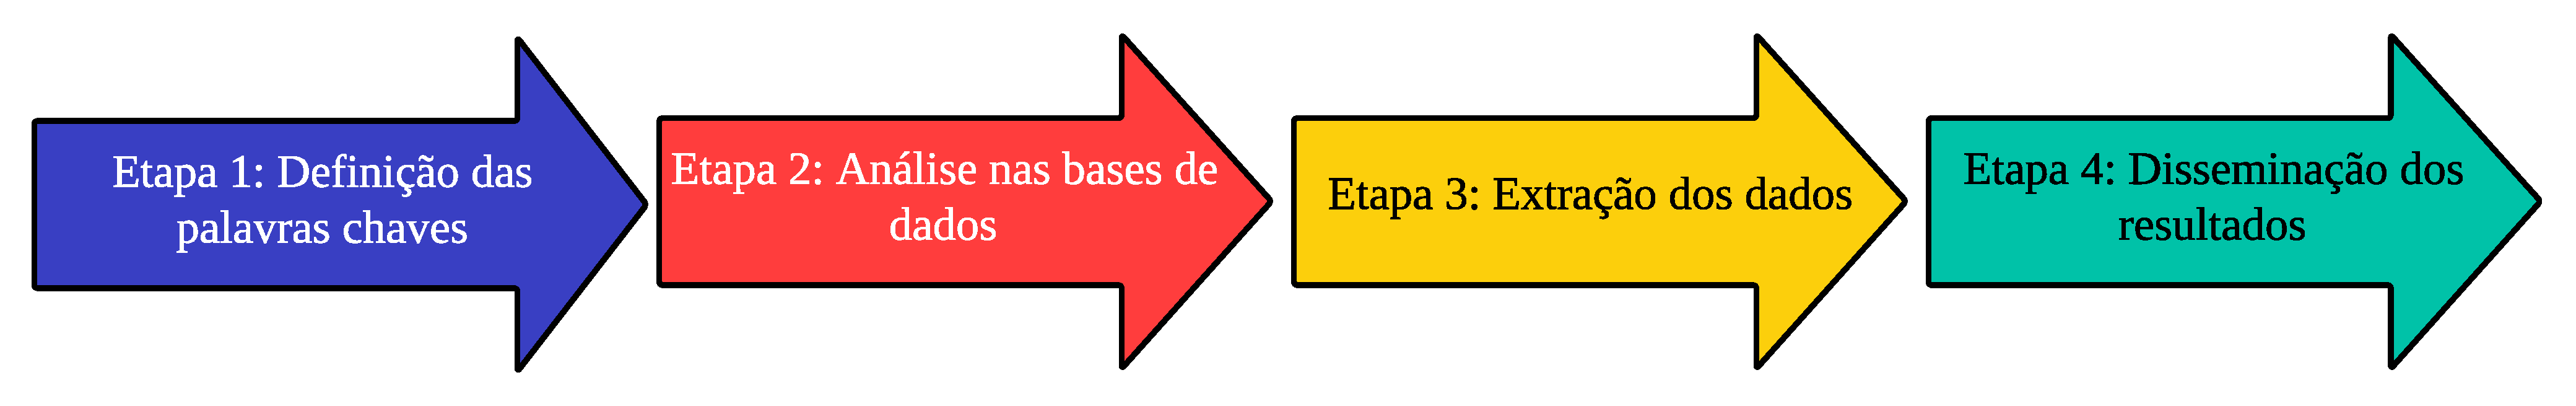
\includegraphics[width=1\linewidth]{Revisao/Figuras/RSL}
%	
%	\fonte{Adaptado de \citeonline{MARTINS201671}}
%\end{figure}
%	
%Para todas as bases de busca, foram considerados os últimos 7 anos, com exceção do Lens, que retornava poucos artigos. Nessa etapa, foram utilizadas palavras-chave que se adequam melhor à pesquisa, como ``\textit{time series forecasting}'', ``\textit{time series analysis}'' e ``\textit{nonlinear forecasting}''.
%	
%No cruzamento das palavras-chave, obteve-se um número considerável de artigos, sem restringir a área em que cada um pode ser publicado. A Tabela \ref{tb1} apresenta a tabulação dos resultados obtidos, sem excluir duplicatas, que serão tratadas na seção \ref{subesec:resul da revisão}.
%	
%Na etapa seguinte, é realizada uma avaliação preliminar de cada artigo obtido, sem aplicar nenhum filtro anual nas buscas. Analisar todos os artigos dessa maneira resultaria em um número elevado, por exemplo, no banco de dados Scopus são 5072 artigos, na Web of Science são 217 artigos, totalizando 5289 artigos sem remover duplicatas. É importante ressaltar que esses artigos passaram apenas pelo filtro de idioma inglês e de serem artigos, visando aprimorar a busca e a tomada de decisões. Ao aplicar o filtro dos últimos 7 anos, obtém-se um número mais gerenciável de artigos para análise. Levando em consideração a diferença entre essa estimativa apresentada na Tabela \ref{tb1} e a quantidade de artigos restantes após a remoção de duplicatas, tem-se menos de 5163 artigos para análise. É válido lembrar que, ao remover as duplicatas, esse número pode diminuir ainda mais, atingindo o objetivo proposto neste trabalho.
%	
%Na etapa final, é realizada uma análise mais aprofundada do conteúdo dos artigos selecionados, levando em consideração as áreas de especialização e correlação com séries temporais. Como esta revisão está inserida no contexto de um programa de mestrado em Engenharia de Produção e Sistemas, vale a pena analisar a correlação com áreas como Matemática. A Figura \ref{fig:areas} mostra que as áreas mais relevantes para a pesquisa são ``Informática'', ``Engenharia'' e ``Matemática'', representando 50\% das publicações. Portanto, a pesquisa está alinhada com a utilização de conceitos matemáticos básicos para realizar uma estimativa do número de artigos.
%	
%
%
%%\subsection{Resultados da Busca de Revis\~ao}\label{subesec:resul da revisão}
%
%
%São apresentados os resultados da pesquisa, utilizando um software para melhor aproveitamento de cada banco de dados utilizado no trabalho. Inicialmente, é realizada uma análise no \textit{software VOSviewer}.
%
%
%A Figura \ref{fig:scopus-09-08} mostra uma lista das palavras mais frequentemente utilizadas como sinônimos ou em conjunto com "time series analysis" nos artigos. A análise da base de dados do Scopus é feita com uma ferramenta que exibe as palavras-chave relacionadas em cada campo de busca, proporcionando uma visão abrangente das correlações com as palavras-chave principais.
%
%\begin{figure}[H]
%	\centering
%	\caption{Palavras-chave mais populares na Scopus}
%	\label{fig:scopus-09-08}
%	\includegraphics[width=0.8\linewidth]{Revisao/Figuras/"scopus 09-08"}
%	
%	\fonte{Elaboração própria a partir de dados da Scopus (2016 a 2022)}
%\end{figure}
%
%Nesse primeiro momento, são obtidas 3.484 palavras-chave, sendo que 212 delas atingem o limite estabelecido. É importante destacar que as palavras-chave base utilizadas são ``\textit{time series forecasting and time series analysis}'' no Scopus.
%
%
%A análise do banco de dados Web of Science, apresentada na Figura \ref{fig:web-09-08}, também é realizada por meio de uma ferramenta que mostra as palavras-chave relacionadas em cada campo de busca. Mais uma vez, é possível obter uma visão ampla das correlações com as palavras-chave principais.
%
%\begin{figure}[H]
%	\centering
%	\caption{Palavras-chave mais populares na Web of Science}
%	\label{fig:web-09-08}
%	\includegraphics[width=0.8\linewidth]{Revisao/Figuras/"web 09-08"}
%	
%	
%	
%	\fonte{Elaboração própria a partir de dados da Web of Science (2016 a 2022)}
%\end{figure}
%
%Nesse primeiro momento, são obtidas 305 palavras-chave, sendo que 13 delas atingem o limite estabelecido. É importante ressaltar que as palavras-chave base utilizadas são \textit{``time series forecasting and time series analysis''} na Web of Science.
%
%
%
%
%
%A Tabela \ref{tb1} apresenta as palavras-chave utilizadas em cada base de dados, juntamente com o número de artigos encontrados inicialmente. No entanto, é importante ressaltar que esses dados ainda não foram processados para remover duplicatas. Após a utilização do \textit{software Mendeley} para eliminar artigos repetidos, restam 308 artigos únicos, os quais serão considerados nesta revisão.
%
%
%\begin{table}[H]
%	\caption{Cruzamento de palavras-chave através da aplicação de filtros de ano e de linguagem}\label{tb1}
%	\centering
%	\begin{tabular}{@{}cp{2cm}p{1cm}p{2cm}p{1cm}p{2cm}p{2cm}p{2cm}@{}}
%		\toprule
%		Bases                             & \multicolumn{5}{c}{Palavras Chaves}                                                         & Resultado \\ \midrule
%		\multirow{3}{*}{Scopus}           & time   series forecasting & AND & time   series analysis    &     &                         & 4956       \\
%		& nonlinear forecasting     & AND & time   series forecasting &     &                         & 75         \\ 
%		& time   series forecasting & AND & time   series analysis    & AND & nonlinear   forecasting & 41        \\ \midrule
%		\multirow{3}{*}{Web   of Science} & time   series forecasting & AND & time   series analysis    &     &                         & 181       \\ 
%		& nonlinear forecasting     & AND & time   series forecasting &     &                         & 22        \\ 
%		& time   series forecasting & AND & time   series analysis    & AND & nonlinear   forecasting & 14        \\ \midrule
%		\multicolumn{6}{c}{Total}                                                                                                       & 5289       \\ \bottomrule
%	\end{tabular}
%	
%	\fonte{Elaboração própria a partir de dados da Scopus, Lens e Web of Science (2016 a 2023)}
%\end{table}
%
%
%
%A Figura \ref{fig:regressao-linear-dos-artigos-baseados-nos-anos} apresenta um gráfico que ilustra a relação entre o número de artigos publicados e os anos correspondentes. Foi realizada uma análise utilizando regressão linear para examinar essa relação ao longo do tempo.
%
%\begin{figure}[H]
%	\centering
%	\caption{Analise das quantidades de artigos em relação aos anos}
%	\label{fig:regressao-linear-dos-artigos-baseados-nos-anos}
%	\includegraphics[width=0.9\linewidth]{Revisao/Figuras/"regressão linear dos artigos baseados nos anos"}
%	
%	\fonte{Elaboração própria a partir de dados da Scopus, Lens e Web of Science (2016 a 2022)}
%\end{figure}
%
%A equação de regressão linear obtida é a seguinte:
%
%\begin{eqnarray}
%	y(x) &=& 8,3571x - 16,803 \quad \text{com } R^2 = 0,3062\label{eq1}
%\end{eqnarray}
%
%Na equação \eqref{eq1}, $y(x)$ representa a equação da reta, onde $x$ é a variável independente que corresponde aos anos. O coeficiente angular da reta é de $ 8,3571$, e o coeficiente linear é de -16.803, indicando o ponto de intersecção com o eixo $y$.
%
%O coeficiente de determinação, $R^2$, é utilizado para avaliar a proporção da variação na variável dependente (número de artigos) que pode ser explicada pela variação na variável independente (anos). Nesse caso, o valor de $R^2$ é de $0,3062$, o que indica que aproximadamente $30,62\%$ da variação nos números de artigos pode ser explicada pela passagem do tempo.
%
%O coeficiente de determinação mede a relação entre a variável dependente e as variáveis independentes, representando a porcentagem da variação explicada pela regressão em relação à variação total. Quando $R^2$ é igual a 1, todos os pontos observados estão exatamente na reta de regressão, indicando um ajuste perfeito, ou seja, todas as variações em $y$ são totalmente explicadas pela variação em $x_n$ através da função especificada, sem desvios em torno da função estimada. Por outro lado, quando $R^2$ é igual a 0, conclui-se que as variações em $y$ são exclusivamente aleatórias e a inclusão das variáveis $x_n$ no modelo não fornece nenhuma informação sobre as variações em $y$.
%
%A fórmula do coeficiente de determinação $R^2$ é dada pela equação:
%\begin{equation}
%	R^{2}=\frac{\left(\sum X \cdot Y-\frac{\sum X \cdot \sum Y}{n}\right)^{2}}{\left[\sum X^{2}-\frac{\left(\sum X\right)^{2}}{n}\right] \cdot\left[\sum Y^{2}-\frac{\left(\sum Y\right)^{2}}{n}\right]}=(r)^{2}\label{eq2}
%\end{equation}
%Na equação \eqref{eq2}, $X$ e $Y$ representam as coordenadas no plano cartesiano, como, por exemplo, o par ordenado $(x,y)$. Na análise realizada com a relação entre o número de artigos e os anos, obteve-se um valor de $R^2=30\%$, o que implica que a linha de regressão é influenciada pelo valor encontrado de $R^2$.
%
%Embora seja uma análise simples da relação entre o número de artigos e os anos, essa é uma validação significativa para observar o teste F de significância, que deve ser sempre inferior a $5\%$, também conhecido como valor-p. Com base nesses valores, é possível analisar o significado da linha de regressão e observar que o ano de 2021 foi o ano em que a maioria dos artigos foi publicada sobre o tema das séries temporais.
%
%\begin{table}[H]
	\centering
	\caption{Fator de impacto}\label{tb2}
	\begin{tabular}{@{}cp{3cm}p{3cm}c@{}}
		\toprule
		Revista cientíica      & Quantidade de plubicação & Qualidade da revista & H-INDEX \\\midrule
		Neurocomputing         & 27                         & Q1                     & 143     \\
		IEEE Access            & 18                         & Q1                     & 127     \\
		Applied Soft Computing & 12                         & Q1                     & 143     \\
		Energies               & 11                         & Q2                     & 93      \\
		Energy                 & 11                         & Q1                     & 343     \\ \bottomrule
	\end{tabular}
	
	
	\fonte{Elaboração própria a partir de dados da Scopus, Lens e Web of Science (2016 a 2022)}
\end{table}
%
%A Tabela \ref{tb2} apresenta as revistas que mais publicaram artigos sobre o tema em questão. É importante destacar que muitas dessas revistas estão localizadas fora do Brasil e têm seus nomes em inglês. No entanto, todas as revistas listadas, incluindo aquelas com um alto fator de impacto, como a categoria Q1, apresentam uma correlação significativa com as áreas de \textbf{informática, engenharia e matemática}.
%
%\begin{table}[H]
%	\centering
%	\caption{Fator de impacto}\label{tb2}
%	\begin{tabular}{@{}cp{3cm}p{3cm}c@{}}
%		\toprule
%		Periódicos      & Quantidade de plubicações & Qualidade do periódico & \textit{h-index} \\\midrule
%		Neurocomputing         & 27                         & Q1                     & 143     \\
%		IEEE Access            & 18                         & Q1                     & 127     \\
%		Applied Soft Computing & 12                         & Q1                     & 143     \\
%		Energies               & 11                         & Q2                     & 93      \\
%		Energy                 & 11                         & Q1                     & 343     \\ \bottomrule
%	\end{tabular}
%	
%	
%	\fonte{Elaboração própria a partir de dados da Scopus, Lens e Web of Science (2016 a 2023)}
%\end{table}
%
%Essa observação ressalta a importância dessas áreas de especialização na pesquisa sobre séries temporais, uma vez que estão fortemente representadas nas principais revistas científicas. Essas revistas desempenham um papel fundamental na disseminação do conhecimento e no avanço do campo, garantindo a qualidade e o impacto dos artigos publicados. Portanto, é valioso direcionar a atenção para essas revistas, uma vez que são reconhecidas como fontes confiáveis e respeitadas dentro da comunidade científica.
%
%
%
%
%%\begin{longtable}{clccccc}
%%	\caption{Table Caption} \\
%%			\hline
%%			Pos & authorKeywords                     & Total & AGR  & ADY  & PDLY & \textit{h-index} \\
%%			\hline
%%			\endfirsthead
%%			
%%			\multicolumn{7}{c}{\tablename\ \thetable{} -- Continuação da Página Anterior} \\
%%			\hline
%%			Pos & authorKeywords                     & Total & AGR  & ADY  & PDLY & \textit{h-index} \\
%%			\hline
%%			\endhead
%%			
%%			\hline
%%			\multicolumn{7}{r}{Continua na próxima página} \\
%%			\endfoot
%%			
%%			\hline
%%			\endlastfoot
%%			1   & machine learning                  & 66    & 1.0  & 16.5 & 50.0 & 24     \\
%%			2   & Forecasting                       & 56    & -2.5 & 8.0  & 28.6 & 25     \\
%%			3   & time series                       & 40    & 0.0  & 7.0  & 35.0 & 17     \\
%%			4   & deep learning                     & 38    & 3.0  & 11.5 & 60.5 & 17     \\
%%			5   & Artificial intelligence           & 30    & 3.5  & 7.0  & 46.7 & 15     \\
%%			6   & Prediction                        & 23    & 1.0  & 5.0  & 43.5 & 12     \\
%%			7   & review                            & 19    & -1.0 & 2.5  & 26.3 & 13     \\
%%			8   & Neural networks                   & 18    & 1.0  & 3.0  & 33.3 & 9      \\
%%			9   & Artificial neural networks        & 17    & 0.5  & 2.5  & 29.4 & 11     \\
%%			10  & time series forecasting           & 17    & 0.5  & 4.5  & 52.9 & 9      \\
%%			11  & Time series analysis              & 16    & 2.0  & 3.5  & 43.8 & 9      \\
%%			12  & Forecast                          & 13    & 1.0  & 3.0  & 46.2 & 4      \\
%%			13  & Remote sensing                    & 12    & -0.5 & 1.0  & 16.7 & 10     \\
%%			14  & climate change                    & 11    & -0.5 & 0.5  & 9.1  & 9      \\
%%			15  & Literature review                 & 10    & 1.0  & 2.5  & 50.0 & 5      \\
%%			16  & Renewable energy                  & 10    & 1.0  & 1.5  & 30.0 & 7      \\
%%			17  & hybrid models                     & 10    & 0.5  & 1.5  & 30.0 & 8      \\
%%			18  & ARIMA                            & 9     & 0.5  & 1.0  & 22.2 & 5      \\
%%			19  & regression                       & 9     & 1.0  & 2.0  & 44.4 & 6      \\
%%			20  & big data                         & 8     & -0.5 & 1.0  & 25.0 & 7      \\
%%			21  & COVID-19                         & 7     & -1.0 & 1.5  & 42.9 & 3      \\
%%			22  & Demand forecasting               & 7     & -0.5 & 1.0  & 28.6 & 5      \\
%%			23  & Forecasting models               & 7     & 0.0  & 0.0  & 0.0  & 7      \\
%%			24  & Smart grid                       & 7     & 0.0  & 2.0  & 57.1 & 5      \\
%%			25  & modelling                        & 7     & 0.0  & 1.0  & 28.6 & 5      \\
%%			26  & neural network                   & 7     & 0.0  & 1.0  & 28.6 & 4      \\
%%			27  & Chaos                            & 6     & 0.0  & 0.5  & 16.7 & 4      \\
%%			28  & Time-series forecasting          & 6     & -2.0 & 1.0  & 33.3 & 4      \\
%%			29  & artificial neural network        & 6     & 0.0  & 1.0  & 33.3 & 4      \\
%%			30  & load forecasting                 & 6     & 0.0  & 1.0  & 33.3 & 6      \\
%%			31  & wind power forecasting           & 6     & -1.0 & 1.0  & 33.3 & 4      \\
%%			32  & Decomposition                    & 5     & 0.5  & 0.5  & 20.0 & 4      \\
%%			33  & Hybrid model                     & 5     & 1.0  & 1.5  & 60.0 & 3      \\
%%			34  & Solar energy                     & 5     & 0.5  & 1.5  & 60.0 & 4      \\
%%			35  & Systematic review                & 5     & 0.0  & 1.0  & 40.0 & 4      \\
%%			36  & Uncertainty                      & 5     & -0.5 & 0.0  & 0.0  & 4      \\
%%			37  & Wind power                       & 5     & 0.0  & 1.0  & 40.0 & 5      \\
%%			38  & modeling                         & 5     & 0.0  & 0.5  & 20.0 & 5      \\
%%			39  & prediction intervals             & 5     & -0.5 & 0.0  & 0.0  & 4      \\
%%			40  & Air pollution                    & 4     & -0.5 & 1.0  & 50.0 & 3      \\
%%			41  & Air quality                      & 4     & -0.5 & 0.5  & 25.0 & 4      \\
%%			42  & Clustering                       & 4     & -0.5 & 0.5  & 25.0 & 4      \\
%%			43  & Computational Intelligence       & 4     & -0.5 & 0.0  & 0.0  & 3      \\
%%			44  & Earth Observation                & 4     & 0.0  & 0.5  & 25.0 & 3      \\
%%			45  & Forecast combination             & 4     & -0.5 & 0.0  & 0.0  & 4      \\
%%			46  & LSTM                             & 4     & 0.0  & 1.5  & 75.0 & 2      \\
%%			47  & Monte Carlo simulation           & 4     & -0.5 & 1.0  & 50.0 & 3      \\
%%			48  & Predictive models                & 4     & 0.0  & 1.5  & 75.0 & 3      \\
%%			49  & Systematic literature review     & 4     & 0.0  & 1.0  & 50.0 & 2      \\
%%			50  & Time series models               & 4     & 0.5  & 1.0  & 50.0 & 3      \\
%%			51  & Tourism demand                   & 4     & 0.0  & 0.0  & 0.0  & 4      \\
%%			52  & Wind speed forecasting           & 4     & 0.0  & 1.0  & 50.0 & 3      \\
%%			53  & exponential smoothing            & 4     & 0.0  & 0.5  & 25.0 & 3      \\
%%			54  & land use                         & 4     & 0.0  & 0.0  & 0.0  & 4      \\
%%			55  & regression analysis              & 4     & 0.0  & 0.0  & 0.0  & 4      \\
%%			56  & stochastic models                & 4     & -0.5 & 0.0  & 0.0  & 3      \\
%%			57  & ARMA                             & 3     & 0.0  & 0.0  & 0.0  & 3      \\
%%			58  & Artificial Neural Network (ANN)   & 3     & -0.5 & 1.0  & 66.7 & 2      \\
%%			59  & China                            & 3     & -0.5 & 0.0  & 0.0  & 2      \\
%%			60  & Citation analysis                & 3     & -0.5 & 0.0  & 0.0  & 3      \\
%%			61  & Complexity                       & 3     & 0.0  & 0.0  & 0.0  & 3      \\
%%			62  & Data mining                      & 3     & 0.0  & 0.5  & 33.3 & 3      \\
%%			63  & Data models                      & 3     & -0.5 & 0.5  & 33.3 & 3      \\
%%			64  & Decision tree                    & 3     & 0.5  & 0.5  & 33.3 & 2      \\
%%			65  & Demand side management           & 3     & 0.0  & 0.5  & 33.3 & 3      \\
%%			66  & Drought                          & 3     & -0.5 & 0.5  & 33.3 & 3      \\
%%			67  & Drought forecasting              & 3     & -0.5 & 0.0  & 0.0  & 3      \\
%%			68  & Ecological forecasting           & 3     & 0.0  & 0.0  & 0.0  & 3      \\
%%			69  & Extreme learning machine         & 3     & -1.0 & 0.0  & 0.0  & 3      \\
%%			70  & Forecasting horizon              & 3     & 0.0  & 0.0  & 0.0  & 3      \\
%%			71  & Forecasting methods              & 3     & 0.0  & 0.5  & 33.3 & 3      \\
%%			72  & Forecasting model                & 3     & 0.5  & 1.0  & 66.7 & 1      \\
%%			73  & Genetic algorithms               & 3     & 0.0  & 0.5  & 33.3 & 2      \\
%%			74  & Judgmental forecasting           & 3     & 0.0  & 0.0  & 0.0  & 3      \\
%%			75  & Kalman filter                    & 3     & -1.0 & 0.0  & 0.0  & 1      \\
%%			76  & Optimization                     & 3     & 0.0  & 0.5  & 33.3 & 3      \\
%%			77  & Persistence                      & 3     & 0.0  & 1.0  & 66.7 & 2      \\
%%			78  & RNN                              & 3     & 0.0  & 0.5  & 33.3 & 2      \\
%%			79  & Renewable energy sources         & 3     & 0.0  & 1.0  & 66.7 & 3      \\
%%			80  & Risk                             & 3     & -0.5 & 0.0  & 0.0  & 3      \\
%%			81  & Risk management                  & 3     & 0.0  & 0.5  & 33.3 & 3      \\
%%			82  & Solar power                      & 3     & 0.0  & 1.0  & 66.7 & 3      \\
%%			83  & Stationarity                     & 3     & 0.0  & 0.0  & 0.0  & 3      \\
%%			84  & Wavelet transform                & 3     & 0.0  & 0.5  & 33.3 & 3      \\
%%			85  & Wind speed                       & 3     & 0.0  & 0.0  & 0.0  & 3      \\
%%			86  & bootstrap                        & 3     & -0.5 & 0.0  & 0.0  & 2      \\
%%			87  & deep neural networks             & 3     & -1.0 & 0.5  & 33.3 & 3      \\
%%			88  & fuzzy logic                      & 3     & -1.0 & 0.0  & 0.0  & 3      \\
%%			89  & hybrid methods                   & 3     & 0.0  & 1.0  & 66.7 & 3      \\
%%			90  & land cover                       & 3     & 0.0  & 0.0  & 0.0  & 3      \\
%%			91  & probabilistic forecasting        & 3     & 0.0  & 0.5  & 33.3 & 3      \\
%%			92  & reliability                      & 3     & 0.0  & 0.0  & 0.0  & 3      \\
%%			93  & robustness                       & 3     & -0.5 & 0.0  & 0.0  & 3      \\
%%			94  & state space                      & 3     & 0.0  & 0.0  & 0.0  & 3      \\
%%			95  & support vector machines          & 3     & 0.5  & 0.5  & 33.3 & 2      \\
%%			96  & time series prediction           & 3     & 0.5  & 1.0  & 66.7 & 2      \\
%%			97  & time-series                      & 3     & -0.5 & 0.5  & 33.3 & 2      \\
%%			98  & time-series analysis             & 3     & 0.5  & 1.0  & 66.7 & 1      \\
%%			99  & water demand                     & 3     & 0.5  & 1.5  & 100.0& 1      \\
%%			100 & weather                          & 3     & 0.5  & 0.5  & 33.3 & 2      \\
%%			\hline
%%\end{longtable}
%
%
%
%
%
%Em resposta à questão colocada anteriormente \eqref{questão:rev1}, foi utilizada a Figura \ref{fig:autores-relacao-entre-artigos-publicados} para visualizar de forma mais clara os autores que mais publicaram sobre o tema em análise. O gráfico apresenta um histograma que destaca os autores cujo número de publicações é maior que 4 durante o período de 2016 a 2022. Essa abordagem visa evitar a inclusão de todos os autores e destacar aqueles que tiveram uma contribuição significativa no campo, considerando o critério estabelecido de pelo menos 4 publicações. Dessa forma, é possível identificar os principais autores que se destacam nesse tópico específico, fornecendo uma visão geral da distribuição da produção científica entre os pesquisadores.
%
%\begin{figure}[htpb!]
	\centering
	\caption{Relação de autores entre artigos publicados}
	\label{fig:autores-relacao-entre-artigos-publicados}
	\includegraphics[width=0.8\linewidth]{Revisao/Figuras/"Autores Relação entre artigos publicados"}
	
	
	\fonte{Elaboração própria a partir de dados da Scopus (2016 a 2022)}
\end{figure}
%
%Na Tabela \ref{tb:autor} apresenta a taxa de crescimento médio (AGR) e documentos médios por ano (ADY) período: 2014 - 2023.
%
%\begin{table}[H]
%	\centering
%	\caption{Tabela de Exemplo}\label{tb:autor}
%	\begin{tabular}{ccccccc}
%		\hline
%		Pos & Author       & Total & AGR  & ADY  & PDLY & \textit{h-index} \\
%		\hline
%		1   & El-Shafie, A. & 4     & 0.0  & 1.0  & 50.0  & 2    \\
%		2   & Liu, H.       & 4     & -0.5 & 0.0  & 0.0   & 4    \\
%		3   & Ahmad, T.     & 3     & 0.0  & 0.0  & 0.0   & 3    \\
%		4   & Ahmed, A.N.   & 3     & 0.0  & 1.0  & 66.7  & 2    \\
%		5   & Chen, C.      & 3     & -0.5 & 0.0  & 0.0   & 3    \\
%		6   & Ozturk, I.    & 3     & 0.0  & 0.0  & 0.0   & 3    \\
%		7   & Tiwari, A.K.  & 3     & 0.0  & 0.0  & 0.0   & 3    \\
%		8   & Wang, Y.      & 3     & -0.5 & 0.0  & 0.0   & 3    \\
%		9   & Yang, D.Z.    & 3     & 0.0  & 0.0  & 0.0   & 3    \\
%		10  & Yaseen, Z.M.  & 3     & 0.5  & 1.0  & 66.7  & 3    \\
%		\hline
%	\end{tabular}
%\end{table}
%
%
%
%
%
%
%
%
%A pergunta de pesquisa \eqref{questão:rev2} foi abordada por meio da análise da Figura \ref{fig:mapa-mundi-artigos}, que apresenta os países com maior número de publicações sobre o assunto em escala, ordenados de forma decrescente. Os principais países que se destacam nessa análise são os seguintes: China, com $119$ publicações; Estados Unidos, com $67$ publicações; Índia, com $57$ publicações; Brasil, com $32$ publicações; Espanha, com $28$ publicações; Reino Unido, com $25$ publicações; Austrália, com $24$ publicações; Irã, com $18$ publicações; Malásia, com $17$ publicações; e Canadá, com $16$ publicações.
%
%\begin{figure}[H]
%	\centering
%	\caption{Mapa mundial da publicação de artigos em todo o mundo}
%	\label{fig:mapa-mundi-artigos}
%	\includegraphics[width=0.87\linewidth]{Revisao/Figuras/"mapa mundi artigos"}
%	
%	
%	\fonte{Elaboração própria a partir de dados da Scopus, Lens e Web of Sicence (2016 a 2022)}
%\end{figure}
%
%É importante ressaltar que o mapa não exibe todos os países e seus respectivos números de publicações, mas destaca aqueles com maior produção nesse contexto específico. Essa análise ajuda a identificar os países com maior contribuição científica nessa área de estudo, fornecendo insights sobre os locais onde a pesquisa sobre séries temporais tem sido mais ativa.
%
%\begin{figure}[htpb!]
	\centering
	\caption{Áreas de aplicação do tema}
	\label{fig:areas}
	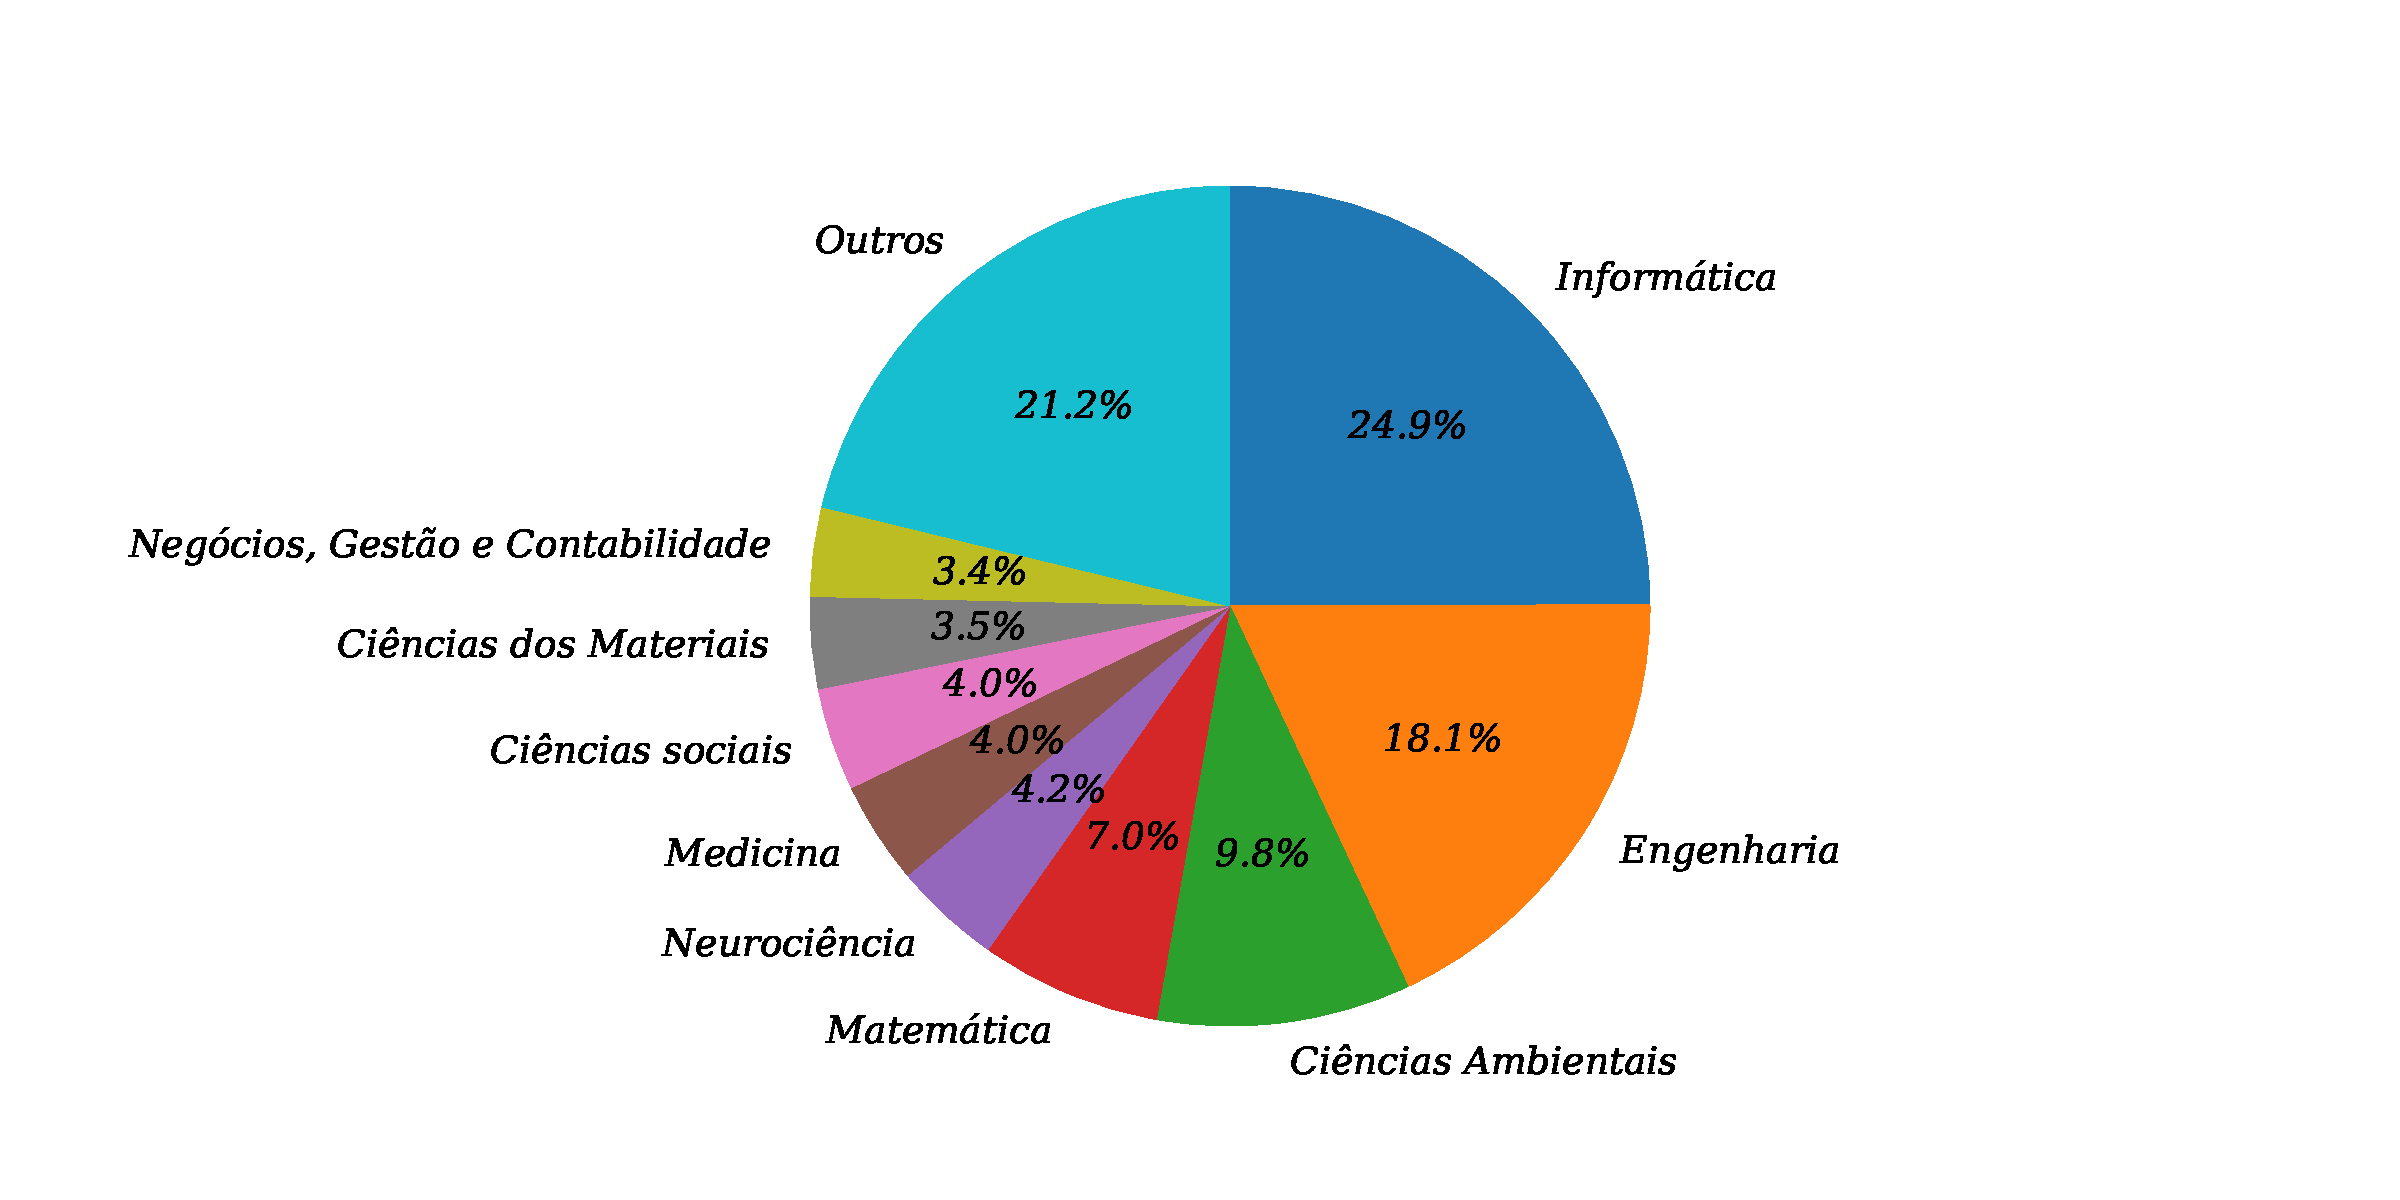
\includegraphics[width=0.9\linewidth]{Revisao/Figuras/areas}
	\vspace{0.2cm}
	
	\fonte{Elaboração própria a partir de dados da Scopus, Lens e Web of Sicence (2016 a 2022)}
\end{figure}

%
%Para responder à pergunta de pesquisa \eqref{questão:rev3}, foi criado um gráfico circular, apresentado na Figura \ref{fig:areas}, que ilustra as áreas com maior número de publicações durante o período analisado na revisão. A Tabela \ref{tb3} complementa o gráfico, fornecendo os valores específicos de cada área e a quantidade de publicações correspondente.
%
%O gráfico circular oferece uma representação visual clara das áreas que se destacam em termos de produção científica no campo das séries temporais. Ao examinar a tabela, é possível identificar as áreas com maior número de publicações, permitindo uma compreensão aprofundada das principais áreas de conhecimento relacionadas ao tema. Essa análise contribui para uma melhor compreensão da distribuição de publicações e áreas de pesquisa ao longo do período estudado.
%
%\begin{table}[!htb]
	\centering
	\caption{Áreas e seus valores respetivos de artigos em cada área.}\label{tb3}
	\begin{tabular}{@{}ll@{}}
		\toprule
		Informática                      & 240 \\ \midrule
		Engenharia                       & 174 \\
		Ciências Ambientais              & 94  \\
		Matemática                       & 67  \\
		Neurociência                     & 40  \\
		Medicina                         & 38  \\
		Ciências sociais                 & 38  \\
		Ciências dos Materias            & 34  \\
		Negócios, Gestão e Contabilidade & 33  \\
		Outros                           & 204 \\ \bottomrule
	\end{tabular}

	
	\fonte{Elaboração própria a partir de dados da Scopus, len e Web of Sicence (2016 a 2022)}
\end{table}
%
%Na última pergunta de pesquisa, referente à \eqref{questão:rev4}, foi realizada uma investigação dos artigos mais influentes na revisão. Esses artigos retratam alguns dos métodos utilizados por renomados autores \citeonline{Golyandina2020, Kumar2021, Xie2019, Lara-Benitez2021, Ahmad2018, CarvalhoJr.2019, Tan2021, Liu2019, Liu2021, Rossi2018, Soyer, Martinovic2020a, Ursu2016, Wang2016, Shih2019a, Moon2019, Chou2018, Bergmeir2018, Boroojeni2017, Chou2018a, Coelho2017, Du2020, Sadaei2019, Salgotra2020, Tyralis2017, Vlachas2020, Yang2019a, Shen2020, Sezer2020, Chen2018, Buyuksahin2019, Li2020, Kulshreshtha2020, Samanta2020, Xu2019, Graff2017, Taieb2016}.
%
%Esses artigos abordam diferentes métodos usados pelos autores para previsão de séries temporais e análise não-linear dessas previsões. Eles representam contribuições significativas para o avanço do conhecimento e aplicação prática das séries temporais, oferecendo insights valiosos sobre abordagens eficazes nesse campo. Ao incluir esses estudos influentes na análise, obtém-se uma visão abrangente dos métodos e técnicas mais relevantes na previsão de séries temporais.
%
%No estudo conduzido por \citeonline{Xu2019}, um modelo híbrido foi proposto, combinando o modelo linear AR e LR com o modelo não-linear ARIMA e o modelo DBN. Essa abordagem permite capturar tanto os comportamentos lineares quanto os não-lineares de uma série temporal. Por outro lado, \citeonline{Li2020} comparou o desempenho de previsão da abordagem MAELS com outros modelos de aprendizado de máquina de última geração, como ANN, CNN, RNN, LSTM, GRU, Transformer, Prophet ARIMA e SVM-VAR. As abordagens ANN, CNN, RNN, GRU, Transformer e LSTM são capazes de lidar com dados multivariados de entrada e saída, enquanto o ARIMA utiliza informações passadas para prever o futuro com base em características como autocorrelação e médias móveis.
%
%\begin{table}[H]
%	\centering
%	\caption{Modelos baseado na literatura e nos artigos}\label{tb:mode}
%	\begin{tabular}{ccccccc}
%		\hline
%		Pos & authorKeywords & Total & AGR  & ADY  & PDLY & \textit{h-index} \\
%		\hline
%		1   & ARIMA          & 230   & -9.0 & 36.0 & 31.3 & 27     \\
%		2   & LSTM           & 182   & 4.5  & 51.5 & 56.6 & 29     \\
%		3   & Transformer    & 44    & 12.0 & 21.0 & 95.5 & 6      \\
%		4   & ANN            & 43    & -1.5 & 5.0  & 23.3 & 16     \\
%		5   & SARIMA         & 42    & -3.0 & 8.0  & 38.1 & 13     \\
%		6   & CNN            & 41    & 1.5  & 11.5 & 56.1 & 13     \\
%		7   & GRU            & 33    & 1.5  & 9.5  & 57.6 & 12     \\
%		8   & RNN            & 28    & 0.5  & 7.0  & 50.0 & 10     \\
%		9   & Random Forest  & 21    & 0.5  & 5.0  & 47.6 & 6      \\
%		10  & Prophet        & 17    & -1.5 & 4.0  & 47.1 & 7      \\
%		11  & XGBoost        & 15    & 2.0  & 5.5  & 73.3 & 6      \\
%		12  & ARMA           & 14    & -1.0 & 1.5  & 21.4 & 8      \\
%		13  & ARIMAX         & 10    & -1.0 & 1.0  & 20.0 & 3      \\
%		14  & SARIMAX        & 8     & 0.0  & 3.0  & 75.0 & 4      \\
%		15  & AR             & 5     & 0.5  & 1.5  & 60.0 & 1      \\
%		\hline
%	\end{tabular}
%	
%	\fonte{Elaboração própria a partir de dados da Scopus e Web of Science}
%\end{table}
%
%Dessa forma, por meio dessa revisão sistemática e análise de conteúdo, a pergunta de pesquisa formulada no início do capítulo foi respondida.
%Além desses modelos mencionados, também será utilizada a versão atualizada do ARIMA nesta dissertação. Os modelos SARIMA e SARIMAX também serão comparados para determinar qual deles é o mais adequado. Além disso, serão empregados os modelos Light GBM e XGBoost.